\chapter{Conception d'Arcus}

\tikzset{
    module/.style={
        rectangle, draw,
        minimum height=1.5em
    }
}

Nous avons commencé par décider d'une architecture globale pour l'application. Cette architecture est résumée dans la vue d'ensemble en figure~\ref{fig:conception-vue-ensemble}.

\begin{figure}[h!]
    \centering
    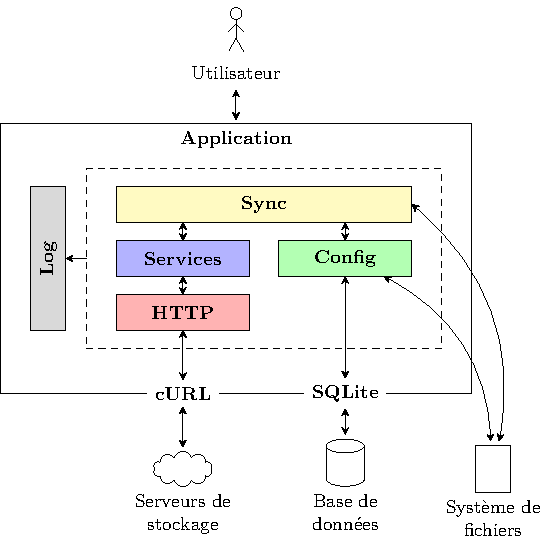
\includegraphics{figures/overview}
    \caption{\textbf{Vue d'ensemble de l'architecture de l'application.} Au centre, dans le cadre «~Application~», sont présentés les différents modules participant à l'architecture de l'application. Le niveau d'abstraction des modules va en croissant vers le haut du schéma. Les flèches représentent les interactions internes à l'application et celles entre les acteurs et ressources externes et l'application.}
    \label{fig:conception-vue-ensemble}
\end{figure}
\clearpage

Notre application a besoin de communiquer avec les interfaces de programmation (ou A.P.I.) des différents services de stockage de fichiers. Ces services fournissent en général une interface de communication utilisant \textit{HyperText Transfer Protocol} (HTTP). C'est un «~protocole applicatif pour les systèmes d'information distribués, collaboratifs utilisant des documents riches~»~\parencite{fielding1999}, donc particulièrement adapté au transfert de documents. Afin de communiquer avec ces services, notre application doit contenir un module de transmission de données sur HTTP, symbolisé par \tikz[baseline=(http.base)]\node[module,fill=red!30] (http) {\small{\textbf{HTTP}}}; dans la vue d'ensemble.

Bien que les fournisseurs de services de stockage connus tels que Nextcloud, OneDrive ou Dropbox utilisent HTTP, ils ont adopté des architectures hétérogènes qui font qu'il est difficile d'écrire un code unique permettant de communiquer avec toutes leurs interfaces. Dans notre application, nous devons donc construire une couche d'abstraction de ces hétérogénéités. Ce module, symbolisé par \tikz[baseline=(service.base)]\node[module,fill=blue!30] (service) {\small{\textbf{Services}}}; dans la vue d'ensemble, s'appuie sur les fonctionnalités du module HTTP.

Comme chaque utilisateur de la machine cliente peut choisir les répertoires qu'il souhaite synchroniser via l'application, la liste de ces répertoires doit être sauvegardée à un endroit de la machine. Ces informations sont regroupées dans une configuration dite locale spécifique à chaque utilisateur. Il existe par ailleurs des informations spécifiques à chaque répertoire synchronisé, comme par exemple la liste des fichiers présents ou la liste des services connectés. Ces informations sont quant à elles regroupées dans une configuration synchronisée sur les différentes machines d'un même utilisateur. Nous avons décidé d'isoler cette fonctionnalité dans un module de configuration, symbolisé par \tikz[baseline=(config.base)]\node[module,fill=green!30] (config) {\small{\textbf{Config}}}; dans la vue d'ensemble.

En s'appuyant sur ces différentes abstractions, nous pouvons mettre en place le moteur de synchronisation, cœur de l'application. Ce moteur doit permettre l'envoi des données contenues dans les répertoires sélectionnés par l'utilisateur vers les services de stockage connectés. Réciproquement, il doit permettre le rapatriement de celles-ci depuis les services distants vers la machine de l'utilisateur. Ce module est symbolisé par \tikz[baseline=(sync.base)]\node[module,fill=yellow!30] (sync) {\small{\textbf{Sync}}}; dans la vue d'ensemble.

Enfin, nous avons décidé qu'il était nécessaire de créer un module de journalisation. Grâce à ce module, les différents composants de l'application seront en mesure d'écrire des informations sur un journal global dans un format unifié. Ce journal global, qui pourra être redirigé vers la sortie standard ou un fichier, aidera au débogage en cas de défaillance de l'application. Dans la vue d'ensemble de l'architecture, il est symbolisé par  \tikz[baseline=(log.base)]\node[module,fill=gray!30] (log) {\small{\textbf{Log}}};.

\section{Transmission des données aux serveurs}

Le module HTTP permet l'échange de données entre un \emph{client} et un \emph{serveur} suivant le protocole HTTP. Ce protocole permet au client d'envoyer des demandes de données au serveur et de recevoir des réponses, mais pas l'inverse : c'est toujours le client qui demande des données au serveur. Pour ce faire, le client formule une requête, composée notamment d'un verbe, d'une \emph{Uniform Resource Locator} (URL) et d'une liste d'en-têtes. Le verbe spécifie l'action qui doit être entreprise sur la ressource désignée par l'URL. Les en-têtes servent à donner plus de détails sur la requête. La norme HTTP/1.1~\parencite{fielding1999} définit les verbes principaux suivants :

\begin{description}
    \item[\texttt{GET} :] récupérer les données contenues dans la ressource désignée par l'URL ;
    \item[\texttt{HEAD} :] récupérer les caractéristiques associées à la ressource désignée par l'URL ;
    \item[\texttt{POST} :] envoyer des données au serveur ;
    \item[\texttt{PUT} :] créer une ressource à l'URL donnée ;
    \item[\texttt{DELETE} :] supprimer la ressource désignée par l'URL.
\end{description}

Une fois la requête formulée par le client dans le module Services, celle-ci est transmise au serveur choisi. Ce serveur doit à son tour formuler une réponse qui satisfait la requête du client et la lui retourner. Ce mode de fonctionnement nous a amené à choisir la modélisation présentée dans la figure~\ref{fig:conception-http} pour le module HTTP.

\begin{figure}[h!]
    \centering
    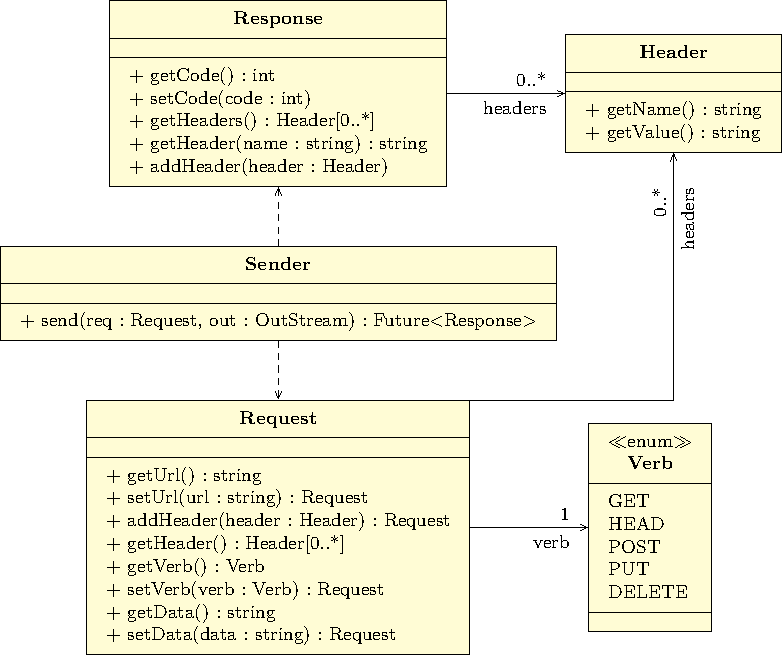
\includegraphics{figures/http}
    \caption{\textbf{Modélisation UML du module HTTP.} La classe \texttt{Sender} est au cœur du module, elle permet d'envoyer des requêtes et d'obtenir de façon asynchrone une réponse de la part du serveur. Cela signifie que le reste de l'application peut continuer à s'exécuter pendant que l'on attend la réponse du serveur à une demande. Ces requêtes doivent préalablement être construites selon le modèle donné par la classe \texttt{Request}. Les réponses fournies par le serveur suivent le modèle de la classe \texttt{Response}.}
    \label{fig:conception-http}
\end{figure}

\section{Définition d'une interface multi-services}

Le module Services a pour but d'abstraire le dialogue avec les interfaces de communication des différents services de stockage. Pour créer ce module, nous avons étudié les interfaces de deux fournisseurs de services majeurs : Dropbox et OneDrive. Nous avons constaté que chaque fournisseur avait une interface qui divergeait de celle de ses concurrents, faute de standard établi.

Par exemple, avec un compte OneDrive, pour obtenir des informations sur le quota alloué et son taux d'utilisation, il faut formuler une requête HTTP avec le verbe \texttt{GET} sur l'URL \url{https://graph.microsoft.com/v1.0/me/drive}~\parencite{onedrive-api}. À l'inverse, avec un compte Dropbox, pour obtenir les mêmes informations, la requête doit utiliser le verbe \texttt{POST} et porter sur l'URL \url{https://api.dropboxapi.com/2/users/get_space_usage}~\parencite{dropbox-api}.

Nous voyons sur ces exemples que les verbes HTTP ou les URL à utiliser pour accéder aux ressources sur les services sont variables.
Toutefois, parmi les services de stockage de fichiers les plus connus, une large majorité a adopté une architecture d'interface de communication dite en \emph{Representational State Transfer} (Rest). Ce type d'architecture, théorisée par \citeauthor{fielding2000} en \citeyear{fielding2000}, repose sur les principes suivants.

\begin{description}
    \item[\textbf{Utilisation sémantique de HTTP.}] L'interface utilise le protocole HTTP décrit dans le module précédent. Elle associe sémantiquement les verbes du protocole à chaque action réalisable ; par exemple, elle utilise le verbe \texttt{GET} lorsqu'il s'agit de récupérer des informations ou \texttt{DELETE} pour en supprimer. Elle utilise les URL pour désigner des ressources et non pas, par exemple, pour désigner une page de connexion.

    \item[\textbf{Échange de requêtes et réponses descriptives.}] Toutes les informations nécessaires au traitement d'une requête du client sont contenues uniquement dans celle-ci. Le serveur n'utilise pas d'informations contextuelles qui seraient liées aux requêtes précédemment effectuées. Il renvoie des réponses descriptives pouvant être traitées en tant que telles sans avoir besoin d'effectuer une requête supplémentaire.

    \item[\textbf{Exclusivité d'accès aux données via le serveur.}] Le serveur est le seul ayant accès à la base de données ou aux informations quelles qu'elles soient. Le client n'y accède que par l'intermédiaire du serveur. Cela simplifie notamment la gestion de la cohérence des données puisque seul le serveur en est responsable.
\end{description}

Les interfaces de OneDrive et Dropbox que nous avons étudiées s'efforcent de suivre ces principes, même s'il subsiste des incompatibilités. Nous avons décidé de profiter du fait que le protocole HTTP soit commun à une très grande majorité des interfaces de communication des services de stockage pour construire notre abstraction. Les incompatibilités nous ont amené à conclure qu'il serait très difficile d'écrire un code unique pour accéder aux différents services.

Nous avons donc créé une interface commune pour accéder à celles des services de stockage, puis réalisé différentes implémentations de cette interface, une par service supporté. Cette modélisation nous permettra d'intégrer plus facilement de nouveaux services par la suite sans devoir modifier le code des autres modules. La figure~\ref{fig:conception-services} présente l'architecture du module Services.

\begin{figure}[h!]
    \centering
    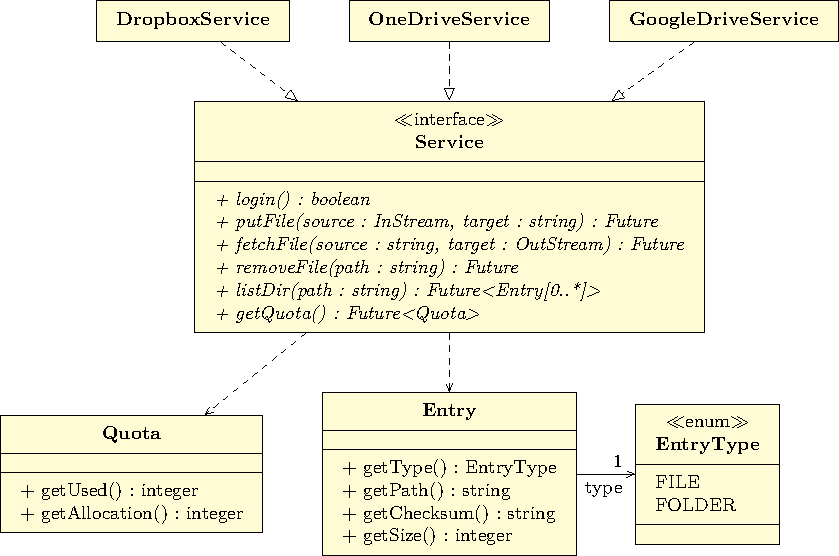
\includegraphics{figures/services}
    \caption{\textbf{Modélisation UML du module Services.} L'interface \texttt{Service} est l'élément principal du module. Elle définit les actions communes que l'application doit être en mesure de réaliser sur chaque service : authentification, ajout d'un fichier, récupération d'un fichier, suppression d'un fichier, listage d'un répertoire, récupération du quota et de son utilisation. Toutes ces actions sont asynchrones.}
    \label{fig:conception-services}
\end{figure}

\section{Configuration locale et configurations synchronisées}

\subsection{Notion de zone de synchronisation}

Nous avons décidé lors de la rédaction du cahier des charges de permettre à l'utilisateur de synchroniser les données d'un ensemble de répertoires (et de leurs sous-répertoires) de son choix. Nous désignerons dans la suite de ce rapport les données de chaque répertoire par l'expression «~zone de synchronisation~».

Ces zones sont associées à un unique répertoire sur la machine de l'utilisateur, situé n'importe où dans son répertoire d'accueil. Elles ne peuvent pas se chevaucher : aucun fichier n'appartient à deux zones de synchronisation.

Pour chaque zone, l'application doit être en mesure de reconstituer les fichiers dispersés en blocs sur les différents services. Pour ce faire, elle a besoin de conserver des informations sur la répartition de ces blocs. Elle a également besoin de pouvoir comparer l'état des zones de la machine actuelle avec celles du serveur, afin de réaliser la synchronisation.

En particulier, nous avons besoin pour chaque bloc de savoir de quel fichier il fait partie, l'ordre dans lequel il apparaît, les services de stockage sur lesquels il est stocké et peut être récupéré. Enfin, l'application a besoin de conserver les informations d'authentification pour chaque service.

\subsection{Conception d'un index d'état}

Pour répondre à ces besoins, nous avons choisi de mettre en place un index d'état pour chaque zone. Cet index est synchronisé avec chaque service de stockage utilisé, afin de pouvoir être récupéré par d'autres machines et servir de base à la reconstitution du répertoire associé. Il contient les informations sur les blocs, les fichiers et les services.

Chaque bloc fait partie d’un unique fichier et possède un identifiant unique indépendant de ce fichier. Il est stocké sur au moins un service. L'index stocke également le \emph{hash} du bloc, correspondant à une somme de contrôle des données qu’il contient, et permettant de savoir si ces données ont changé. Enfin, chaque bloc possède un numéro d’ordre qui indique la position qu’il occupe dans le fichier original relativement aux autres.

Chaque fichier et chaque répertoire possède un identifiant unique indépendant de son chemin. Nous avons décidé d'utiliser une structure récursive pour stocker l'arborescence de la zone de synchronisation, dans laquelle chaque fichier ou répertoire est lui-même fils d'un autre répertoire. Chaque fichier possède un nom et contient au moins un bloc.

Enfin, les comptes de services de stockage que l'utilisateur a connectés à la zone sont stockés dans l'index. Ces comptes contiennent un ensemble de blocs de fichiers synchronisés. L'application conserve le nom du fournisseur du service en question ainsi que les informations d'authentification. Dans cette première modélisation de l'application, nous conservons les informations d'authentification en clair dans l'index, nous ne tenons donc pas compte de leur sécurité. Nous réglerons ce problème dans le futur en chiffrant l'index.

En raison de la complexité de la structure de l'index, nous avons choisi de le stocker sous forme d'une base de données relationnelle, dont le modèle entité-association est présenté en figure~\ref{fig:conception-base}.

\begin{figure}[h!]
    \centering
    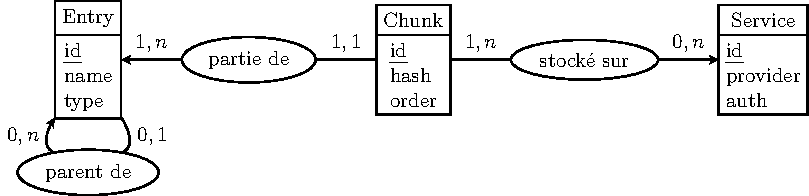
\includegraphics{figures/base}
    \caption[Modèle entité-association de la base de données de l'index]{\textbf{Modèle entité-association de la base de données pour l'index.}}
    \label{fig:conception-base}
\end{figure}

De ce fait, nous avons choisi de considérer chaque zone de synchronisation comme une entité totalement indépendante, possédant sa propre configuration synchronisée avec différents services, sous forme d'une base de données.

Sur cet aspect, notre conception s'apparente à celle du logiciel Git qui définit des \emph{dépôts}, semblables à nos zones de synchronisation, qui contiennent leur propre index~\parencite{rosenberg2010} et sont synchronisés avec un serveur distant. Nous divergeons cependant sur le fait que Git se concentre sur l'aspect de gestion de versions des données, ce que notre application ne prend pas en compte car cela ne correspond pas aux objectifs que nous nous sommes fixés.

Ce choix permet une plus grande flexibilité pour l'utilisateur. En effet, si nous avions choisi de centraliser le stockage des informations d'authentification des services de toutes les zones de synchronisation dans un seul fichier, il n'aurait par exemple pas été possible de synchroniser une zone avec deux services particuliers et une autre avec deux différents.

En choisissant de stocker le plus d'informations possible dans une configuration spécifique à chaque zone, l'application peut non seulement fonctionner dans le cas où ces zones ne partagent pas les mêmes services, mais également dans le cas où elles les partagent.

\subsection{Conception d'une configuration locale}

Comme expliqué avant, les zones de synchronisation sont associées, sur une machine, à un répertoire racine. Si l'on synchronise cette zone avec une autre machine, il y a de fortes chances pour que l'on souhaite l'associer à un répertoire ayant un chemin différent. Par exemple, le nom de l'utilisateur peut avoir changé entre les deux machines, ou elles peuvent ne pas fonctionner sur le même système d'exploitation.~\footnote{Le système Windows place par exemple le répertoire d'accueil de l'utilisateur dans \texttt{C:\textbackslash{}Users\textbackslash{}utilisateur} alors que les dérivés de GNU/Linux utilisent généralement \texttt{/home/utilisateur}.}

Pour gérer ces cas, nous avons décidé de créer un fichier de configuration local sur chaque machine et pour chaque utilisateur. Ce fichier contient les paramètres qui n'ont pas lieu d'être partagés par plusieurs machines.

Dans cette configuration, pour le moment seule la liste des associations entre chaque zone de synchronisation et son répertoire racine pour la machine actuelle est stockée. Nous pourrons y inclure plus de paramètres si le besoin se présente dans le futur. La figure~\ref{fig:conception-syncdir} montre un exemple de mise en place de ces différentes configurations sur un système GNU/Linux.

\begin{figure}[h!]
    \centering
    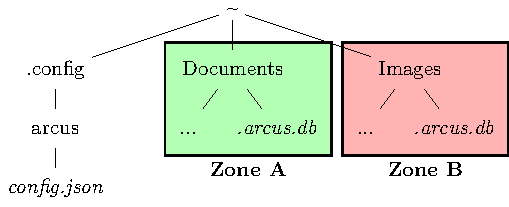
\includegraphics{figures/syncdir}
    \caption{\textbf{Exemple de répartition des différentes configurations de l'application.} Les fichiers dont le nom est en italique contiennent les configurations de l'application telles que décrites dans les parties précédentes. La configuration locale, unique pour l'utilisateur, est stockée dans \texttt{\textasciitilde{}/.config/arcus/config.json}. Dans cet exemple, l'utilisateur a choisi de synchroniser deux zones, A associée aux répertoire des documents et B associée aux répertoire images. Dans chacune de ces zones, la base de données est stockée dans le fichier \texttt{.arcus.db}.}
    \label{fig:conception-syncdir}
\end{figure}

\subsection{Gestion des configurations dans l'application}

Notre application doit ainsi gérer deux configurations, une configuration synchronisée spécifique à chaque zone, et une configuration locale pour chaque utilisateur, qui est dépendante de la machine utilisée. Pour ce faire, nous avons conçu un module de configuration dont la modélisation est présentée en figure~\ref{fig:conception-config}.

\begin{figure}[h!]
    \centering
    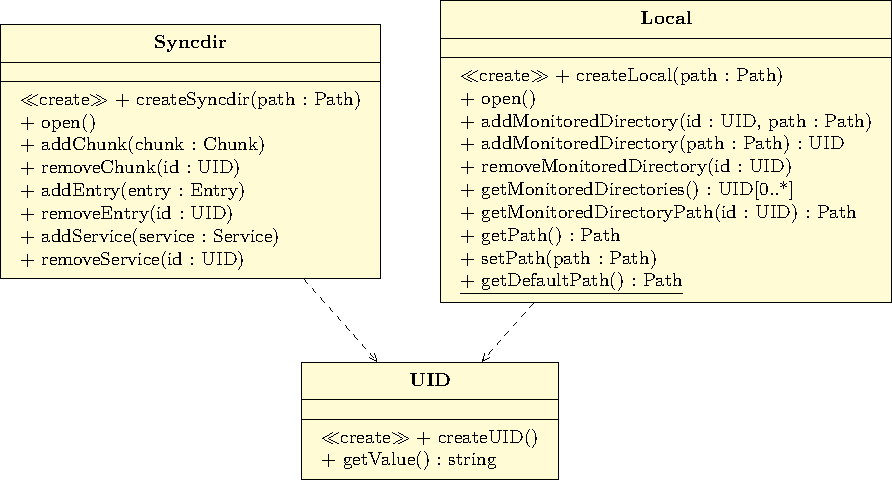
\includegraphics{figures/config}
    \caption{\textbf{Modélisation UML du module Config.} La classe \texttt{Local} permet la lecture et l'écriture de la configuration locale et la gestion des associations entre les zones de synchronisation et leur répertoire. La classe \texttt{Syncdir} permet de gérer la base de données associée à une zone particulière. Enfin, la classe \texttt{UID} permet la génération d'identifiants uniques, utilisés pour identifier les fichiers, les zones de synchronisation, les blocs et les services.}
    \label{fig:conception-config}
\end{figure}

\section{Moteur de synchronisation des fichiers}

Le moteur de synchronisation constitue la partie principale de l'application. Il s'appuie sur les fonctionnalités et les abstractions construites dans les modules précédents. Son rôle est de s'assurer que les zones de synchronisation locales et sur le serveur restent synchronisées.

Pour ce faire, il observe les changements effectués par l'utilisateur dans les zones de synchronisation locales à sa machine. À chaque changement local, il téléverse les données vers les serveurs distants en les répartissant. Réciproquement, à chaque changement distant, il télécharge les données et reconstitue les fichiers en local.

Lors de cette procédure de synchronisation, nous distinguons trois cas qui peuvent se présenter.

\begin{description}
    \item[Modification locale sans modification distante.] Ce cas est le plus courant. Il se produit lorsque des changements locaux sont effectués sur une machine et qu'aucune modification n'est effectuée entre temps sur les serveurs.

    \item[Modification distante sans modification locale.] Ce cas ne peut se produire que lorsqu'au moins deux machines sont synchronisées avec les mêmes serveurs. Par exemple, si un utilisateur effectue des changements sur une machine B et les envoie sur les serveurs, et qu'aucune modification n'est effectuée sur une machine A. Alors, dans le référentiel de la machine A, il y a eu des changements distants sans modification locale.

    \item[Modification locale et distante.] Ce cas est le plus problématique, et ne peut se produire que lorsqu'au moins deux machines sont synchronisées avec les mêmes serveurs. Par exemple, si un utilisateur effectue des changements sur une machine A et une machine B, que les changements de la machine B sont envoyés en premier et que la machine A cherche à se synchroniser. Alors, dans ce cas, dans le référentiel de la machine A, il y a eu des changements distants et des changements locaux, il y a donc conflit.
\end{description}

Chacun de ces trois cas doit être traité par une procédure différente. Le moteur doit donc être en mesure de distinguer les trois cas afin d'enclencher la bonne procédure.

Pour discriminer ces cas, nous avons choisi d'utiliser un numéro de version, stocké dans la base de données de chaque zone. Ce numéro est fixé à 0 initialement. À chaque modification ce numéro est incrémenté, avant d'envoyer les changements vers le serveur. Un algorithme permettant de discriminer les trois cas en utilisant le numéro de version est présenté dans la figure~\ref{fig:conception-sync-discr}.

\begin{figure}[h]
    \centering
    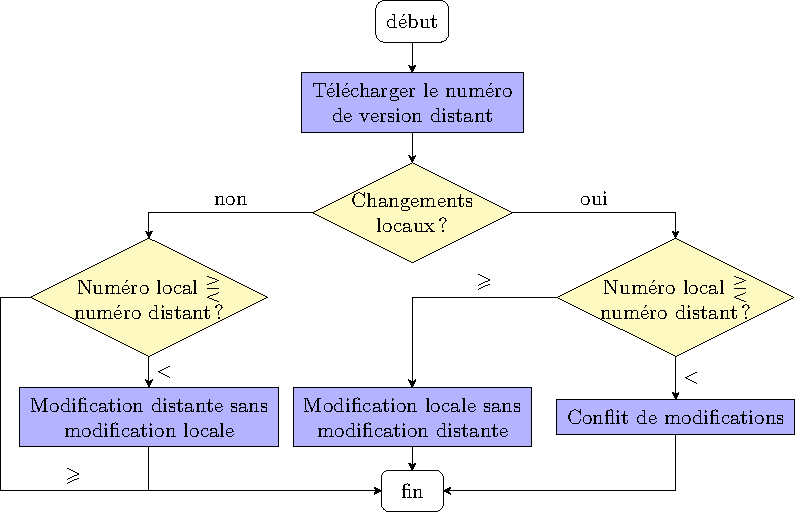
\includegraphics{figures/sync-discr}
    \caption{\textbf{Algorithme de discrimination des différents cas de synchronisation.} Dans le cas où il y a des changements locaux, alors, si le numéro local est strictement inférieur au numéro distant, on se trouve dans le cas où il y a des modifications locales sans modification distante. Sinon, il y a un conflit de modifications. À l'inverse, s'il n'y a pas de modificaiton locale, alors il y a des modifications distantes seulement si le numéro local est strictement inférieur au numéro  distant. Sinon, il n'y a rien à faire.}
    \label{fig:conception-sync-discr}
\end{figure}

Cependant, il persiste un cas ambigu : si le numéro de version distant est incrémenté entre le moment où nous le téléchargeons depuis le serveur et le moment où nous le comparons dans l'algorithme. Dans la version initiale d'Arcus, nous avons décidé de ne pas traiter ce cas pour simplifier le traitement, mais nous le traiterons toutefois dans le futur.

\section{Journal des actions de l'application}

Comme nous l'avons détaillé précédemment, l'application est responsable de la synchronisation de plusieurs répertoires, d'échanges de données avec des serveurs, de la gestion de configurations... Ces fonctionnalités sont souvent complexes, et nous avons anticipé le fait que lorsque des bogues se produiront à l'exécution, ils seront éventuellement difficiles à résoudre.

Pour pallier ce problème, nous avons décidé de créer un journal des actions de l'application. Celui-ci permet de retranscrire précisément la séquence d'actions effectuée par l'application, d'identifier plus facilement les problèmes éventuels et de remonter à la source de ceux-ci.

Nous avons pour cela décidé d'associer à chaque message du journal la date et l'heure à laquelle il a été produit. Cette date est formattée en ISO 8601~\parencite{iso8601} pour éviter toute ambiguïté et faciliter son interprétation par d'autres applications. Nous avons attribué à chaque message un niveau de sévérité (informatif, avertissement ou erreur) et un code couleur qui permettent de relever facilement les informations importantes. Enfin, la ligne de code ayant produit un message lui est clairement associée afin de pouvoir diagnostiquer plus facilement les éventuels problèmes. La figure~\ref{fig:conception-journal} résume le format que nous avons choisi pour les messages du journal.

\begin{figure}[h!]
    \centering
    \begin{tikzpicture}[font=\ttfamily, node distance=0cm]
        \node (date-heure)
            {\textcolor{black!70}{YYYY-MM-DD}T\textcolor{black!70}{HH:MM:SS}};

        \node[right=of date-heure] (niveau)
            {[\textcolor{green!80!black}{info}|\textcolor{orange!80!black}{warn}|\textcolor{red!80!black}{err!}]};

        \node[right=of niveau] (source)
            {\textcolor{black!70}{fichier}:\textcolor{black!70}{ligne}};

        \node[right=of source] (sep) { - };

        \node[right=of sep] (message)
            {\textcolor{black!70}{Message}};

        \tikzset{font=\rmfamily\itshape}

        \node[below=of date-heure] {Date et heure};
        \node[below=of niveau] {Sévérité};
        \node[below=of source] {Source};
    \end{tikzpicture}

    \caption{\textbf{Format unifié d'écriture des messages pour le journal de l'application.}}
    \label{fig:conception-journal}
\end{figure}
